\documentclass{article}
\usepackage{a4}
\usepackage{rotating}
\usepackage{epsfig}

\newcommand{\degrees}{\mbox{${}^{\circ}$}}
\newcommand{\htt}{\mbox{$3_{10}$}}
\newcommand{\tick}{\mbox{$\surd$}}

\title{The ups and downs of protein topology; rapid comparison of protein
structure} 
\author{Andrew C.R.\ Martin}

\begin{document}
\maketitle

%%%%%%%%%%%%%%%%%%%%%%%%%%%%%%%%%%%%%%%%%%%%%%%%%%%%%%%%%%%%%%%%%%%%%%%%%
\begin{abstract}
Protein topology can be described at different levels. At the most
fundamental level, it is a sequence of secondary structure elements
(``primary topology string''). Searching predicted primary topology
strings against a library of strings from known protein structures is
the basis of some protein fold recognition methods.  Here a method
known as TOPSCAN is presented for rapid comparison of protein
structures. Rather than a simple 2-letter alphabet (encoding strand
and helix), more complex alphabets are used encoding direction,
proximity, accessibility and length of secondary elements and loops in
addition to secondary structure.  Comparisons are made between the
structural information content of primary topology strings and
encodings which contain additional information (``secondary topology
strings'').  The algorithm is extremely fast, with a scan of a large
domain against a library of more than 2000 secondary structure strings
completing in around 30 seconds.
\end{abstract}

%%%%%%%%%%%%%%%%%%%%%%%%%%%%%%%%%%%%%%%%%%%%%%%%%%%%%%%%%%%%%%%%%%%%%%%%%
\section{Introduction}
As new structure data becomes available, the classification of protein
folds is becoming more and more important. When a new structure is
solved, one wishes to ask the question of whether this fold has been
seen before. If the fold is one of the commonly occuring superfolds
(e.g.\ immunoglobulin-fold, TIM barrel, $\alpha\beta$-plait, Rossman
fold), then it can generally be recognised by eye, but the less common
folds are more difficult to recognise. Automated servers to answer
this question have recently been developed and rely on structure
comparison programs.

Unfortunately, detailed automatic structure comparison is a
time-consuming process. The double-dynamic programming algorithm used
in SSAP at the atomic coordinate level is particularly computer
intensive making it impractical to run a full scan of a protein of any
size against a library of known folds.  An experimental
``CATH-server'' at UCL has made use of sequence screening and a
hierarchical expansion scheme through the representative levels in the
CATH domain classification database to reduce the search, but in the
worst case scenario, it could still be necessary to scan against more
than 2000 near-identical sequence representatives. We estimate
approximately 2 weeks of computer time would be required to scan a
large protein domain such as a TIM barrel in this way and this is
clearly impractical for use as a server. Our goal therefore is to
develop a rapid method for protein fold comparison.

The CATH classification of protein domain structures is a hierachical
classification encoding class (C), architecture (A), topology (T),
homology (H), sequence family (S), near-identical sequence (N),
identical sequence (I). The use of the word ``topology'' in this
description is somthing of a misnomer. When we refer to the topology
of a protein fold, what we generally mean is the three-dimensional
fold. i.e.\ given a particular spatial arrangement of secondary
structure elements, the topology describes how these elements are
connected.

The dictionary definition of ``topology'' is the factors which remain
unchanged as an object undergoes a continuous deformation.  In terms
of secondary structure elements, the true topology is simply the
sequence of secondary structure elements.  i.e.\ if one imagines a
protein as a piece of string with beads representing the secondary
structures along the string, straightening the string or folding it up
will not change the topology.  Here, we describe this as the ``primary
topology'', while the protein fold is described as the ``tertiary
topology''. A primary topology string is a sequence of E and H
characters (representing $\beta$-strand and $\alpha$-helix in Kabsch
and Sander, DSSP, notation).

When a sequence for a protein of unknown structure does not show
obvious sequence homology with a protein of known structure, fold
recognition is commonly used to give clues as to the three-dimensional
structure. There are two common approaches to this problem: one is
``threading'' which assesses how well a sequence is accomodated within
a three-dimensional structure; the other is alignment of a predicted
sequence of secondary structure elements against a fold library
encoded in this form.  These fold recognition methods are therefore
making the assumption that the tertiary topology can be predicted from
the primary topology. We present an analysis of the occurrence of
given primary topologies in different tertiary topologies.

Since primary topology strings can be used for fold recognition, it
should also be possible to use them for three-dimensional structure
comparison.  However, given the extra information available within a
three-dimensional structure, we are able to introduce an intermediate
level of topology ``secondary topology'' which contains additional
information (secondary structure element direction, proximity,
accessibility and length of the elements and the loops which connect
them) to improve the mapping between these lower levels of topological
description and ``tertiary topology'' (i.e.\ protein fold).

TOPSCAN was initially developed as a simple method to reduce the
search space for the CATH-server. In that implementation, the secondary
topology strings contain only the directional information.  It is used
to sort domains and SSAP is then used to make the final selection
working down the TOPSCAN-sorted list. In this way, we can be sure that
we will not miss any hits which might otherwise have been found using
a full search with SSAP alone.


%%%%%%%%%%%%%%%%%%%%%%%%%%%%%%%%%%%%%%%%%%%%%%%%%%%%%%%%%%%%%%%%%%%%%%%%%
\section{Methods}
TOPSCAN reduces a protein to a topology string which can represent the
structure as a string of letters encoding simply the primary topology
(a 2-letter alphabet) or the secondary topology using various
additional data from the 3D structure. For example, by encoding
direction information with the secondary structure, a 12-letter
alphabet is used.

A simple Needleman and Wunsch dynamic programming algorithm is then
applied to compare two such strings and a score for the similarity is
calculated. Alternatively, a library of these topology strings may be
pre-built from the Protein Databank (or a representative subset) and a
structure may then be scanned against this library.

%11111111111111111111111111111111111111111111111111111111111111111111111
\subsection{Datasets}
All analysis was performed using a non-homologous dataset derived from
the CATH classification of protein domain folds. Representative
structures are assigned at T, S and N levels. The representatives from
the N level (Nreps) from CATH v1.6 were selected, but from this set,
any structures now obsoleted from the protein databank and any NMR
structures were removed. This gave a set of **** domains used for all
further analysis.


%11111111111111111111111111111111111111111111111111111111111111111111111
\subsection{Creating primary topology strings}
TOPSCAN enables secondary structure to be calculated from a
three-dimensional structure using either DSSP or STRIDE (for the
analyses presented in this paper, STRIDE was used).  From these
assignments, regions of $\beta$-sheet (Kabsch and Sander assignment,
E) and of $\alpha$-helix (Kabsch and Sander assignment, H) are
extracted. Only continuous regions of at least a specified number of
residues with the same assignment are selected.  This produces the
primary topology of the protein equivalent to a string of E and H
characters. The program also allows one to treat \htt\ helix
assignments as $\alpha$-helix.

%11111111111111111111111111111111111111111111111111111111111111111111111
\subsection{Creating secondary topology strings}
To increase the information content of the topology string, various
information from the three-dimensional structure can be incorporated
into a secondary topology string. 

For simplicity, topology strings are described here as vectors of
characters. In practice, integer vectors are used to allow more than
52 descriptors. This also provides a technical simplification as
lookups in the scoring matrix may be made simply by the integer values
of the two descriptors being compared.

%22222222222222222222222222222222222222222222222222222222222222222222222
\subsubsection{Secondary structure element direction}
The end-points of each secondary structure element in the primary
topology are found and the vector between them is calculated. The
direction of the vector is grouped into one of 6 classes depending on
the largest component of the vector (i.e.\ positive or negative $x$,
$y$, or $z$). This is equivalent to saying the element points up,
down, left, right, forward, or back. The encoding is summarised in
Table~\ref{tab:encoding}.

\begin{table}
\begin{center}
\begin{tabular}{llll} \hline
\multicolumn{2}{c}{Direction} & \multicolumn{2}{c}{Secondary Structure}\\ \cline{3-4}
          &         & strand & helix  \\ \hline
$+y$      & Up      & A      & G      \\
$+x$      & Right   & B      & H      \\
$-y$      & Down    & C      & I      \\
$-x$      & Left    & D      & J      \\
$+z$      & Back    & E      & K      \\
$-z$      & Forward & F      & L      \\ \hline
\end{tabular}
\end{center}
\caption{\label{tab:encoding}Encoding scheme used to represent
          secondary structure and direction information}
\end{table}


Two topology strings are compared using a simple Needleman and Wunsch
dynamic programming algorithm. A scoring matrix is used in the
comparison based on the scoring scheme shown in
Table~\ref{tab:matrix}. The scoring scheme is somewhat arbitrary, but
appears to work well.  In essence, the same secondary structure in the
same orientation scores highest. Different orientations score worse
and different secondary structure types achieve much lower scores.

The starting premise was that for the same type of secondary
structure, one wishes to assign 3 scores: 
\begin{center}
\begin{tabular}{rlll}
\multicolumn{2}{l}{Angle between vectors}&\hspace{1cm}& Direction  \\
0\degrees   & $\le\Delta\le 45\degrees$     && Approximately the same \\
45\degrees  & $\le\Delta\le 135\degrees$    && Approximately right angles \\
135\degrees & $\le\Delta\le 180\degrees$    && Approximately opposite \\
\end{tabular}
\end{center}
\noindent Arbitrarily, these were assigned as scores of 10, 5 and 2
respectively. However, because of the boolean definition of whether a
vector is in a given quadrant, it is possible that vectors actually
point in very similar directions although they are in different
quadrants (for example one points at $+$89\degrees\ while another
points at $+$91\degrees). Picking pairs of random numbers between
0--90 and 90--180 and plotting the distribution of the differences
shows an upside down V shaped curve centred around 90
(data not shown). Two vectors in adjacent quadrants will
actually be within 90\degrees\ of one another 50\% of the time. The
actual score for adjacent quadrants is therefore the median of 10 and
5 ($7.5$ rounded up to 8).

%\begin{figure}
%\centerline{\epsfig{file=dist90.ps}}
%\caption{\label{fig:dist}Distribution obtained by picking 100000 pairs
%of numbers between 0--90 and 90--180 and plotting the differences.}
%\end{figure}

When two vectors are assigned to opposite quadrants, they can never be
closer than 90\degrees. Picking pairs of random numbers between 0--90
and 180--270 gives an identical distribution centred around 180. The
angle between two vectors can never be greater than 180\degrees, so
every angle $<$180\degrees\ observed between vectors in opposite
quadrants can also be seen in vectors assigned to adjacent quadrants.
In opposite quadrants, the angle between two vectors is
$<$135\degrees\ (our cutoff for saying two vectors are approximately
at right angles) $12.5$\% of the time. We therefore assign the score
as $2+((5-2)\times 12.5/100) = 2\frac{3}{8}$ which we round back down
to 2.

For different secondary structure types, we make the simple arbitrary
assignments of 3, 1 and 0.

%% %% %% %% %% %% %% %% %% %% %% %% %% %% %% %% %% %% %% %% %% %% %% %% 
%% This really should be 3,2,0 - simply by applying the rule to the  %%
%% previous scores of ((3/8) * (x-2)) : such that we scale them to   %%
%% have 3 as a maximum score and 0 as a minimum.                     %%
%% %% %% %% %% %% %% %% %% %% %% %% %% %% %% %% %% %% %% %% %% %% %% %% 

% \begin{table}
% \begin{center}
% \begin{tabular}{rrrrrrrrrrrrr}
%   & A & B & C & D & E & F & G & H & I & J & K & L \\
% A &10 & 8 & 2 & 8 & 8 & 8 & 3 & 1 & 0 & 1 & 1 & 1 \\
% B & 8 &10 & 8 & 2 & 8 & 8 & 1 & 3 & 1 & 0 & 1 & 1 \\
% C & 2 & 8 &10 & 8 & 8 & 8 & 0 & 1 & 3 & 1 & 1 & 1 \\
% D & 8 & 2 & 8 &10 & 8 & 8 & 1 & 0 & 1 & 3 & 1 & 1 \\
% E & 8 & 8 & 8 & 8 &10 & 2 & 1 & 1 & 1 & 1 & 3 & 0 \\
% F & 8 & 8 & 8 & 8 & 2 &10 & 1 & 1 & 1 & 1 & 0 & 3 \\
% G & 3 & 1 & 0 & 1 & 1 & 1 &10 & 8 & 2 & 8 & 8 & 8 \\
% H & 1 & 3 & 1 & 0 & 1 & 1 & 8 &10 & 8 & 2 & 8 & 8 \\
% I & 0 & 1 & 3 & 1 & 1 & 1 & 2 & 8 &10 & 8 & 8 & 8 \\
% J & 1 & 0 & 1 & 3 & 1 & 1 & 8 & 2 & 8 &10 & 8 & 8 \\
% K & 1 & 1 & 1 & 1 & 3 & 0 & 8 & 8 & 8 & 8 &10 & 2 \\
% L & 1 & 1 & 1 & 1 & 0 & 3 & 8 & 8 & 8 & 8 & 2 &10 \\
% \end{tabular}
% \end{center}
% \caption{\label{tab:fullmatrix} Full scoring matrix for the 12-letter
% alphabet encoding protein topology.}
% \end{table}

\begin{table}
\begin{center}
\begin{tabular}{lll}\hline
                        & \multicolumn{2}{c}{Secondary structure} \\ \cline{2-3}
Orientation             & Same  & Different     \\ \hline
Same                    & 10    & 3             \\
Off by 1 quadrant       & 8     & 1             \\
Off by 2 quadrants      & 2     & 0             \\ \hline
\end{tabular}
\end{center}
\caption{\label{tab:matrix} Scoring scheme employed in the matrix for
the dynamic programming comparison of two topology strings.}
\end{table}



Because any pair of proteins is in an arbitrary relative orientation,
the definition of ``up'' in one protein may not correspond to ``up''
in the second. Therefore, one of the strings is permuted 23 times,
such that the dynamic programming algorithm comparison is performed a
total of 24 times (equivalent to the 6 sides of a cube, each of which
may be 4 ways up). Table~\ref{tab:permute} shows the modifications
made to the encoding to achieve rotations about $x$, $y$ and $z$ axes.

\begin{table}
\begin{center}
\begin{tabular}{llll}\hline
        & \multicolumn{3}{c} {Rotation axis} \\ \cline{2-4}
        & $x$           & $y$           & $z$           \\ \hline
Old     & ABCDEFGHIJKL  & ABCDEFGHIJKL  & ABCDEFGHIJKL  \\
New     & EBFDCAKHLJIG  & AECFDBGKILJH  & BCDAEFHIJGKL  \\ \hline
\end{tabular}
\end{center}
\caption{\label{tab:permute} Modifications made to topology strings to
        achieve rotations about the $x$, $y$ and $z$ axes.}
\end{table}




%22222222222222222222222222222222222222222222222222222222222222222222222
\subsubsection{Secondary Structure Element Proximity}
To add information about the packing of secondary structure elements,
the proximity of a secondary structure element to the element
precceding it is encoded. This is performed as follows (see
Figure~\ref{fig:proximal}).

\begin{figure}
\centerline{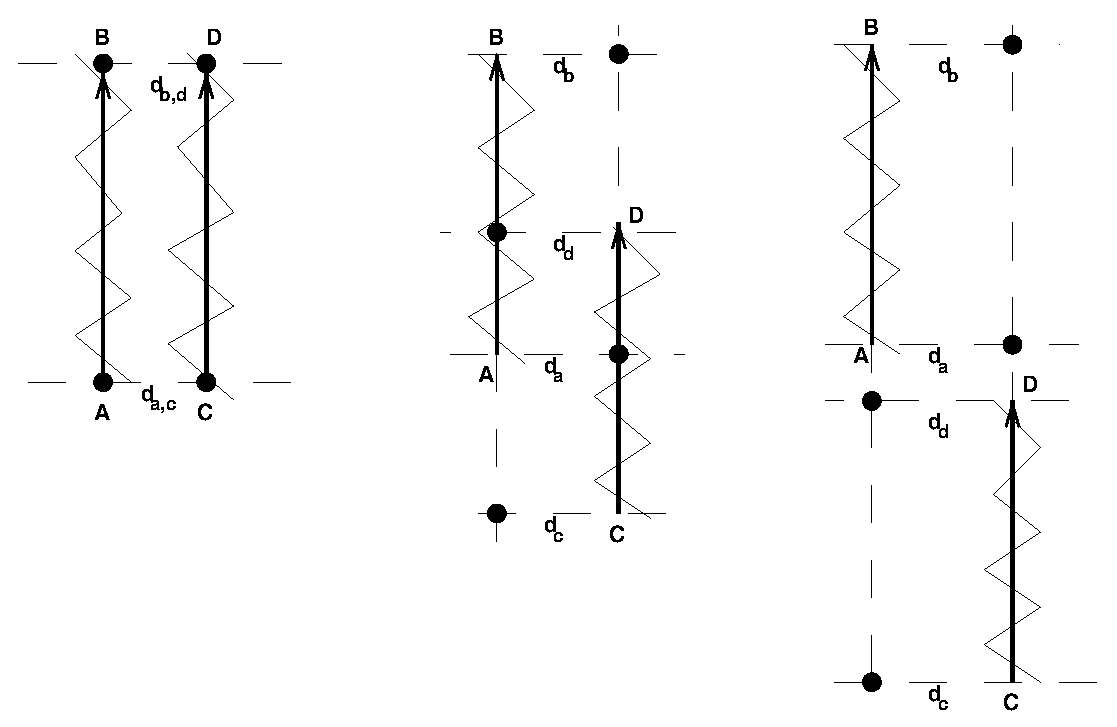
\psfig{file=neighbour.eps,width=\linewidth}}
\caption{\label{fig:proximal}Calculation of proximity of a secondary
structure element to the preceeding element. a) and b) both show
arrangements considered proximal where 
$d_{\mbox{\scriptsize min}} < ***\AA$. 
In c) the elements are not considered proximal.}
\end{figure}

Given an element with endpoints C,D and a preceeding element with
endpoints A,B, the minimum distances between points A and B and the
line described by CD is calculated.  This is repeated with points C
and D to line AB. As each minimum point-to-line distance is calculated
the position on the line closest to the point is calculated. If this
point is between the two endpoints of the line and the distance is
$<***$\AA, then we say that the element C,D is proximal to the
preceeding element and encode this within the topology strings. The
N-terminal element does not have a proximity parameter assigned to
it. 

% \begin{table}
% \begin{center}
% \begin{tabular}{llll} \hline
% \multicolumn{2}{c}{Direction} & \multicolumn{2}{c}{Secondary Structure}\\ \cline{3-4}
%           &         & strand & helix  \\ \hline
% $+y$      & Up      & M      & S      \\
% $+x$      & Right   & N      & T      \\
% $-y$      & Down    & O      & U      \\
% $-x$      & Left    & P      & V      \\
% $+z$      & Back    & Q      & W      \\
% $-z$      & Forward & R      & C      \\ \hline
% \end{tabular}
% \end{center}
% \caption{\label{tab:encoding2}Encoding scheme used to represent
%           secondary structure and direction information where the
%           element is proximal to the preceeding element.}
% \end{table}

The scores in the similarity matrix are multiplied by 0.75 and rounded
to the nearest integer for mismatches in proximity. This also applies
to the other items encoded in secondary topology strings. Note that
all cutoffs use single values, so the penalty of a mismatch (a
reduction of the score by 25\%) is only small.


%22222222222222222222222222222222222222222222222222222222222222222222222
\subsubsection{Accessibility}
Using the same non-redundant fold library, the mean residue
accessibility was calculated for all residues in helices and in
strands as assigned by STRIDE. Secondary structure elements with mean
residue accessibilities less than this mean cutoff (helices:
***\AA${}^{2}$ strands: ***\AA${}^2$) are assigned as burried, others
are exposed.

%22222222222222222222222222222222222222222222222222222222222222222222222
\subsubsection{Element length}
Mean helix and strand lengths were calculated on the same basis. The
mean helix length is *** residues while the mean strand length is ***
residues. These are used as cutoffs to define `long' or `short' elements.

%22222222222222222222222222222222222222222222222222222222222222222222222
\subsubsection{Loop length}
Mean loop lengths are calculated in the same way and assigned to the
element which follows the loop. The first secondary structure element
therefore does not have a loop length parameter assigned to it. The
mean loop length was *** residues.





%11111111111111111111111111111111111111111111111111111111111111111111111
% \subsection{Application within a classification protocol}
% A CATHServer is being developed which allows the automatic
% classification of a novel protein domain in the CATH hierachy.
% TOPSCAN is employed within this protocol where no sequence hit is
% found or where a sequence hit has been found but the SSAP score is
% poor. TOPSCAN is then used to rank all the near-identical sequence
% representatives (NREPs) for similarity to the probe domain. FAST-SSAP
% (which works by comparing secondary structure vectors using
% double-dynamic programming rather than by considering residue-level
% environment vectors as is done with the full version of SSAP) is then
% used to work down this ranked list. If a score better than 60 is
% obtained with FAST-SSAP, the comparison is performed again using the
% full version of SSAP. As soon as a full SSAP comparison achieves a
% SSAP score of at least 70 with at least 60\% overlap of the
% structures, the search is stopped and this structure is reported as
% being the best hit. It is, of course, possible that there are better
% hits farther down the TOPSCAN-ranked list, but this is a necessary
% trade-off of computer time for absolute accuracy of results.





%%%%%%%%%%%%%%%%%%%%%%%%%%%%%%%%%%%%%%%%%%%%%%%%%%%%%%%%%%%%%%%%%%%%%%%%%
\section{Results and Discussion}
%\input results.tex
%\input best.tex
%\input worst.tex
%\input bars.tex

\subsection{Assignment of Secondary Structure (primary topology)}
The assignment of secondary structure is the critical first stage. We
have found that the DSSP algorithm can be over-sensitive to errors in
the structure. For example, NMR structures often show little secondary
structure in DSSP assignments whereas an intuitive visual inspection
shows substantial secondary structure. 

The STRIDE software from Argos and co-workers was designed to reduce
this sensitivity. However, using STRIDE in place of DSSP makes little
difference to the overall results (results not shown). The TOPSCAN
software allows either DSSP or STRIDE secondary structure assignments
to be used.

% The simplified secondary structure assignment scheme used within
% Rasmol actually appears to perform better in assigning secondary
% structures in an intuitive manner and we are investigating the
% possibility of extracting this code from Rasmol for stand-alone
% secondary structure assignment.

We explored the effects of setting the minimum required number of
consecutive residues assigned to a given secondary structure to 3 and
4 residues. We also looked at treating \htt\ helix residues as the
same as $\alpha$-helix (data not shown). This made little difference
when the length cutoff was set to 4, but made results significantly
worse when the length cutoff was set to 3. Presumably this is because
most instances of true \htt\ helix are $\le 3$ residues in length.


\subsection{Does primary topology predict protein fold?}
Using the CATH classification, each protein fold containing more than
one near-identical sequence family (i.e.\ each CAT level containing
more than one Nrep) was examined. Within each of these groups, the
TOPSCAN score was calculated using only the primary topology
(secondary structure cutoff length set to 3). The frequency of scores
obtained is shown in Figure~\ref{fig:primary}a. Unsurprisingly, the
highest peak if for a score of 95--100\%, i.e.\ within a protein fold,
the primary topology is generally identical.

Each protein fold was then compared with every other protein fold in
the same way (Figure~\ref{fig:primary}b). The fifth highest peak in
the distribution is the 95--100\% peak. Initially this appears
surprising. However when one considers, for example, 4-helix bundles,
it becomes obvious that there are multiple folds containing the same
set of secondary structure elements. Thus, by knowing only the primary
topology (perhaps from secondary structure prediction), there is a
high chance of matching the incorrect protein fold with an identical
primary topology.


\begin{figure}
\caption{\label{fig:primary}a) Frequency of scores achieved using
primary topology within a given protein fold b) Frequency of scores
achieved using primary topology when comparing a given fold with every
other fold.}
\end{figure}

\subsection{Assignment of secondary topology}
In addition to secondary structure and the direction of secondary
structure elements, we considered the following factors in defining
secondary topology: accessibility, proximity, element length and loop
length. The performance is assessed in terms of percent coverage vs.\
percent error, specifically taking error rates of 1\% and 5\%. These
results are summarised in Table~\ref{tab:summary}

\begin{table}
\begin{tabular}{|lllll|ll|} \hline
SS length &               &           & Element & Loop   & \multicolumn{2}{c|}{Coverage} \\ \cline{6-7}
cutoff    & Accessibility & Proximity & length  & length & 1\% error & 5\% error \\ \hline
3         &               &           &         &        &           &           \\
3         &               &           &         & \tick  &           &           \\
3         &               &           & \tick   &        &           &           \\
3         &               &           & \tick   & \tick  &           &           \\
3         &               & \tick     &         &        &           &           \\
3         &               & \tick     &         & \tick  &           &           \\
3         &               & \tick     & \tick   &        &           &           \\
3         &               & \tick     & \tick   & \tick  &           &           \\
3         & \tick         &           &         &        &           &           \\
3         & \tick         &           &         & \tick  &           &           \\
3         & \tick         &           & \tick   &        &           &           \\
3         & \tick         &           & \tick   & \tick  &           &           \\
3         & \tick         & \tick     &         &        &           &           \\
3         & \tick         & \tick     &         & \tick  &           &           \\
3         & \tick         & \tick     & \tick   &        &           &           \\
3         & \tick         & \tick     & \tick   & \tick  &           &           \\
4         &               &           &         &        &           &           \\
4         &               &           &         & \tick  &           &           \\
4         &               &           & \tick   &        &           &           \\
4         &               &           & \tick   & \tick  &           &           \\
4         &               & \tick     &         &        &           &           \\
4         &               & \tick     &         & \tick  &           &           \\
4         &               & \tick     & \tick   &        &           &           \\
4         &               & \tick     & \tick   & \tick  &           &           \\
4         & \tick         &           &         &        &           &           \\
4         & \tick         &           &         & \tick  &           &           \\
4         & \tick         &           & \tick   &        &           &           \\
4         & \tick         &           & \tick   & \tick  &           &           \\
4         & \tick         & \tick     &         &        &           &           \\
4         & \tick         & \tick     &         & \tick  &           &           \\
4         & \tick         & \tick     & \tick   &        &           &           \\
4         & \tick         & \tick     & \tick   & \tick  &           &           \\ \hline
\end{tabular}
\caption{\label{tab:summary}Summary of effects of adding information
to the secondary topology strings.}
\end{table}


\subsection{Does secondary topology predict protein fold?}
As with comparison of primary topology, each protein fold containing
more than one near-identical sequence family. Within each of these
groups, the TOPSCAN score was calculated using only the secondary
topology using a secondary structure length cutoff of 3 and including
accessibility, proximity, element length and loop length information 
(Figure~\ref{fig:secondary}a). The distribution is similar to that
seen using primary topology although the scores are generally reduced.

Comparison between protein folds (Figure~\ref{fig:secondary}b) now
peaks at a score of (***) 50--55\% and the very high scoring peaks are
now removed.

Interestingly both the comparisons of primary and secondary topology
within a fold show two comparisons with very low scores. These
structures were examined using RasMol. One pair (domain 3 from PDB
files 1dar and 1elo) are shown in Figure~\ref{fig:1dar1elo}. Whereas
1dar contains only $\beta$-strands, 1elo has two poorly defined
strands and a helix. The sequences of these two are identical, yet the
fold is different. The structures are poorly defined in this region
and this may represent alternative folding of the same domain, or may
simply reflect errors in the structure {*** check the original papers
***}

{*** The other pair.... ***}


\subsection{Problems}
The algorithm has problems in discriminating, for example, a TIM
barrel from a Rossmann fold. These are topologically somewhat similar
--- in both cases, they consist of a core of $\beta$-sheet with
helices on the outside. In the case of the TIM barrel the
$\beta$-sheet is curved into a barrel where as the Rossmann fold has a
relatively flat sheet. Because the differences between the two occur
in a plane perpendicular to the direction of the secondary structure
elements, the current method does not distinguish reliably between these
architectures. 

%% %% %% %% %% %% %% %% %% %% %% %% %% %% %% %% %% %% %% %% %% %% %% %% 
%% Give examples of topology strings for TIM and Rossmann            %%
%% %% %% %% %% %% %% %% %% %% %% %% %% %% %% %% %% %% %% %% %% %% %% %% 

\section{Comparison of TOPSCAN with other rapid methods}
Two methods similar in principle to TOPSCAN are FAST-SSAP and the
constraint-programming methods based on TOPS
diagrams\cite{David_Gilbert_David_Westhead}.  FAST-SSAP uses
double dynamic programming to align vectors representing the secondary
structure elements to compare two structures. The constraint-based
method uses a 4-letter alphabet to represent the two types of
secondary structure going either up or down and adds information about
chirality and hydrogen bonds between secondary structure elements.
Comparison is performed by finding a maximum common template and
scoring the two structures against that template.  The approach taken
by TOPSCAN is unlikely to give results as good as either of these two
methods since the representation is so much simpler. However, this
does allow a very significant speed advantage. It is approximately
25$\times$ faster than the current implementation of FAST-SSAP and
10$\times$ faster than constraint-programming.  FAST-SSAP could be
speeded significantly by pre-calculating all the secondary structure
vectors and by calculating these vectors simply from the end-points of
the secondary structure elements rather than using an Eigenvector.

%% %% %% %% %% %% %% %% %% %% %% %% %% %% %% %% %% %% %% %% %% %% %% %% 
%% Check the timings                                                 %%
%% %% %% %% %% %% %% %% %% %% %% %% %% %% %% %% %% %% %% %% %% %% %% %% 

Compared with FAST-SSAP, the simple segregation of secondary structure
vectors into six quadrants throws away a lot of more detailed
information about the relative orientation of the elements, but as a
result, allows us to perform normal single dynamic programming
removing the need for double dynamic programming.

Compared with the constraint-programming method, our representation
actually has more information about directionality of the secondary
structure vectors, but loses the proximity information (encoded in the
constraint programming by hydrogen-bond information) and the chirality
arcs. 

\section{Conclusion}
TOPSCAN has proved a useful addition to the available methods for
comparing protein structures. In particular, it provides a useful
rapid method of ranking structures for further more detailed
comparison using SSAP. In common with the fast version of SSAP which
relies on secondary structure vectors, TOPSCAN is most likely to fail
when a structure is poorly defined and DSSP or STRIDE are unable to
make reliable secondary structure assignments.

\section{Acknowledgements}
I would like to thank Christine Orengo and Janet Thornton for making
the CATH data available and for their support during the first part of
this work which was funded by departmental funds at UCL as part of the
development of the CATHServer. 

\end{document}



